\section{Conceptual Modelling}\label{sec:cm}

\begin{figure}[h]

\centering
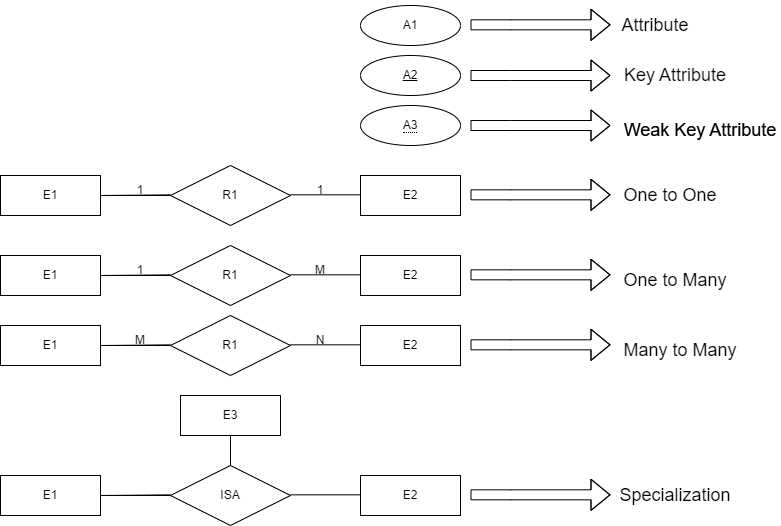
\includegraphics[scale=.5]{info1u}

\caption{Legends}
\end{figure}

\clearpage

\begin{figure}[h]

\centering
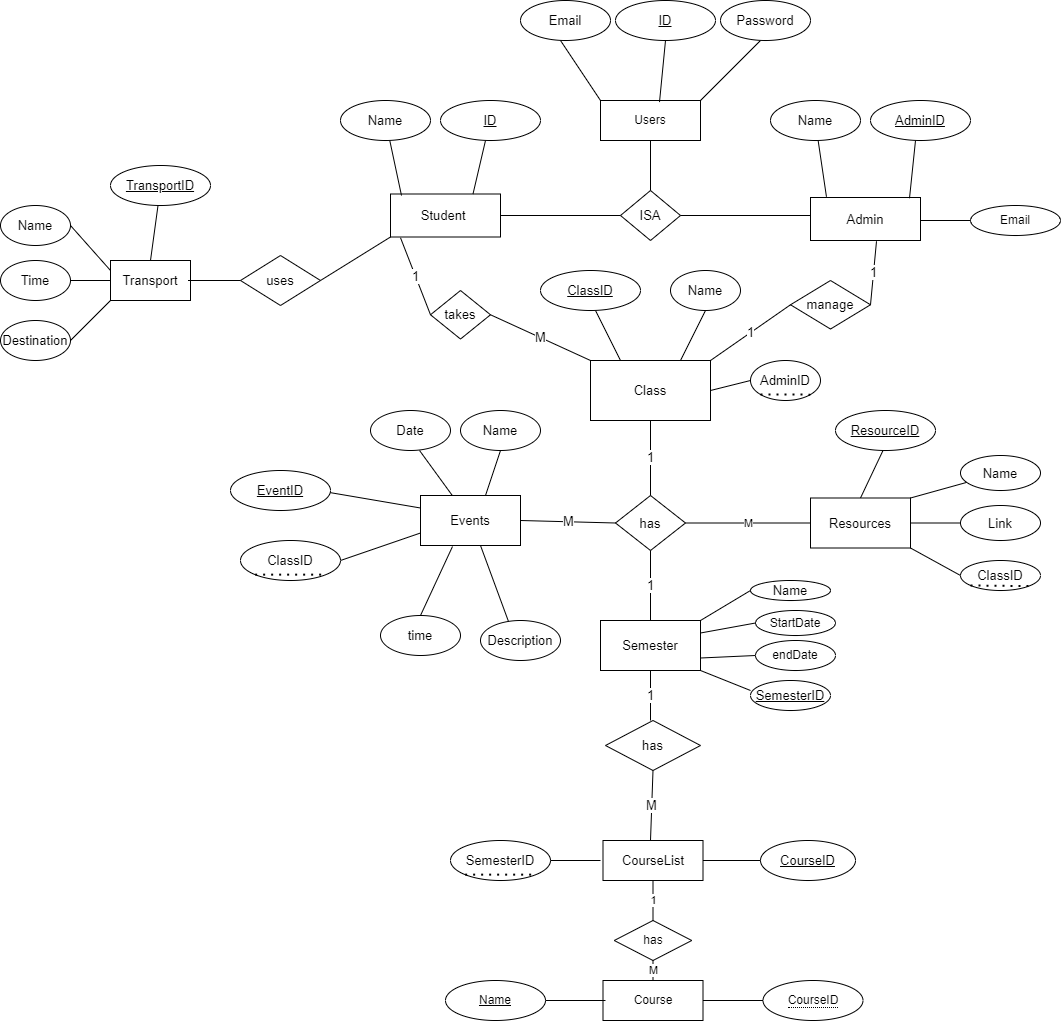
\includegraphics[scale=.4]{er2}

\caption{The E-R diagram for virtual classroom }
\end{figure}
 
 

The E-R diagram for the Virtual Classroom Android App project is as follows:

\begin{itemize}

\item The entity types in the diagram are users , Student, Class, admin , Semester, Course, Resource, Event, and Transport.

\item The relationships between the entities are:
    \begin{itemize}
   \item  Student is takes in one class (Many-to-one relationship)
   \item Class has one Admin (One-to-One relationship)
   \item Class has one Semester (One-to-One relationship)
   \item Semester includes one or more courses (One-to-Many relationship)
   \item Class has one or more resources (One-to-Many relationship)
   \item Class has one or more upcoming events (One-to-Many relationship)
   \item students use transports(Many to Many relationship) 
   \item semester has courseList (One-to-Many relationship)
    \end{itemize}
  \item The attributes of each entity are:
   \begin{itemize}
   \item Users: Email,ID,Password 
   \item Student: ID, Name 
   \item Class: ClassID, Name, AdminID ,SemesterID
   \item Admin: ID, Name, Email 
   \item Semester: semesterID, Name, Start Date, End Date 

  \item Resource: ResourceID, Name,Link, ClassID
  \item Event: EventID, Name, Date, ClassID, Description,time 
  \item Transport: TransportID, Name, time , Destination
  \item courseList: courseID,semesterID 
  
  
   \end{itemize}

\end{itemize}

The E-R diagram was created by first identifying the key entities in the system, which include Students, Classes, ClassRepresentative, Semester, Course, Resource, Event, and Transport. The relationships between these entities were then identified, such as a student being enrolled in one or more classes, and a class having one ClassRepresentative. The attributes of each entity were also identified, such as a student having an ID, name, email, phone number, and profile picture. The E-R diagram was then created by visually representing these entities, relationships, and attributes using the standard ER notation.
